\documentclass[a0paper,portrait]{baposter}


\usepackage{wrapfig}
\usepackage{lmodern}
\usepackage{xcolor}

\usepackage[utf8]{inputenc} %unicode support
\usepackage[T1]{fontenc}


\selectcolormodel{cmyk}

\graphicspath{{figures/}} % Directory in which figures are stored


\newcommand{\compresslist}{%
\setlength{\itemsep}{0pt}%
\setlength{\parskip}{1pt}%
\setlength{\parsep}{0pt}%
}

\newenvironment{boenumerate}
  {\begin{enumerate}\renewcommand\labelenumi{\textbf\theenumi.}}
  {\end{enumerate}}

\usepackage{amsmath}
\usepackage{palatino}
\usepackage{mathpazo}
\usepackage{fontawesome}
\usepackage{hyperref}

\newcommand{\mail}		[1]{\faEnvelope \quad {#1}}
\newcommand{\github}	[1]{\faGithub \quad {#1}}


\begin{document}


\definecolor{Black}{RGB}{0,0,0}
\definecolor{White}{RGB}{255,255,255}

% Basic colors
\definecolor{SeaGreen}{RGB}{111,189,165}
\definecolor{Cyan}{RGB}{0,166,214}
\definecolor{DarkBlue}{RGB}{34,70,122}
\definecolor{Purple}{RGB}{36,46,131}
\definecolor{Turquoise}{RGB}{50,154,179}
\definecolor{SkyBlue}{RGB}{130,187,206}

% Accent colors
\definecolor{Lavender}{RGB}{121,150,180}
\definecolor{Orange}{RGB}{216,130,62}
\definecolor{WarmPurple}{RGB}{110,50,122}
\definecolor{Fuchsia}{RGB}{178,72,146}
\definecolor{BrightGreen}{RGB}{183,200,34}
\definecolor{Yellow}{RGB}{247,234,151}
\definecolor{Pink}{RGB}{138,75,129}
\definecolor{Purple}{RGB}{69,48,117}

\definecolor{customBlockColor}{RGB}{111,189,165}
\definecolor{customAlertColor}{RGB}{31,112,173}
\begin{poster}
{
grid=false,
headerborder=open, % Adds a border around the header of content boxes
colspacing=1em, % Column spacing
bgColorOne=white, % Background color for the gradient on the left side of the poster
bgColorTwo=white, % Background color for the gradient on the right side of the poster
borderColor=WarmPurple, % Border color
headerColorOne=Pink, % Background color for the header in the content boxes (left side)
headerColorTwo=Pink, % Background color for the header in the content boxes (right side)
headerFontColor=white, % Text color for the header text in the content boxes
boxColorOne=white, % Background color of the content boxes
textborder=rounded, %rectangle, % Format of the border around content boxes, can be: none, bars, coils, triangles, rectangle, rounded, roundedsmall, roundedright or faded
eyecatcher=false, % Set to false for ignoring the left logo in the title and move the title left
headerheight=0.11\textheight, % Height of the header
headershape=rounded, % Specify the rounded corner in the content box headers, can be: rectangle, small-rounded, roundedright, roundedleft or rounded
headershade=plain,
headerfont=\Large\textsf, % Large, bold and sans serif font in the headers of content boxes
textfont=\textsf, % Uncomment for paragraph indentation
linewidth=2pt % Width of the border lines around content boxes
}
{}
%
%---------------------------------------------------------------------------
%	TITLE AND AUTHOR NAME
%---------------------------------------------------------------------------
%
{
\color{WarmPurple}\textsf %Sans Serif
{When MAML Learns Quickly Does It Generalize Well?}
} 
%
{\sf\vspace{0.5em}\\
O. Taylan Turan*, David M.J. Tax*, and Marco Loog*
\vspace{0.1em}\\
\small{Pattern Recognition Laboratory, Delft University of Technology, Van Mourik Broekmanweg 6, Delft 2628 XE, The Netherlands
}
\large{
\vspace{0.2em}\\
 \color{WarmPurple}\mail{o.t.turan@tudelft.nl} 
\hspace{0.2em}
  \github{github.com/taylanot}}
}
%
{}

\headerbox{1. Introduction}{name=intro,column=0,row=0, span=2}
{
  \begin{itemize}
    \color{Pink} \item \color{Black} Meta-learning: leverages similar learning problems (tasks) for a specific similar data-scarce target learning problem (task).

    \color{Pink}\item \color{Black} MAML: tackles meta-learning problems by providing an initialization for model parameters that facilitates quick adaptation and good generalization.
  \color{Pink} \item AIM : \color{Black} Investigating the effect of gradient step limitation.
  \end{itemize}
  
}

  \headerbox{2. MAML\begin{NoHyper}\cite{finn2017}\end{NoHyper}}{name=maml,column=2, span=1}
{
  \begin{itemize}
    \color{Pink} \item \color{Black} From $M$ tasks $\{\mathcal{T}_i\}_{i=0}^{M}$
    \color{Pink} \item \color{Black} Learn a model initialization $\bar{\mathbf{w}}_{\text{meta}}$
  \end{itemize}
  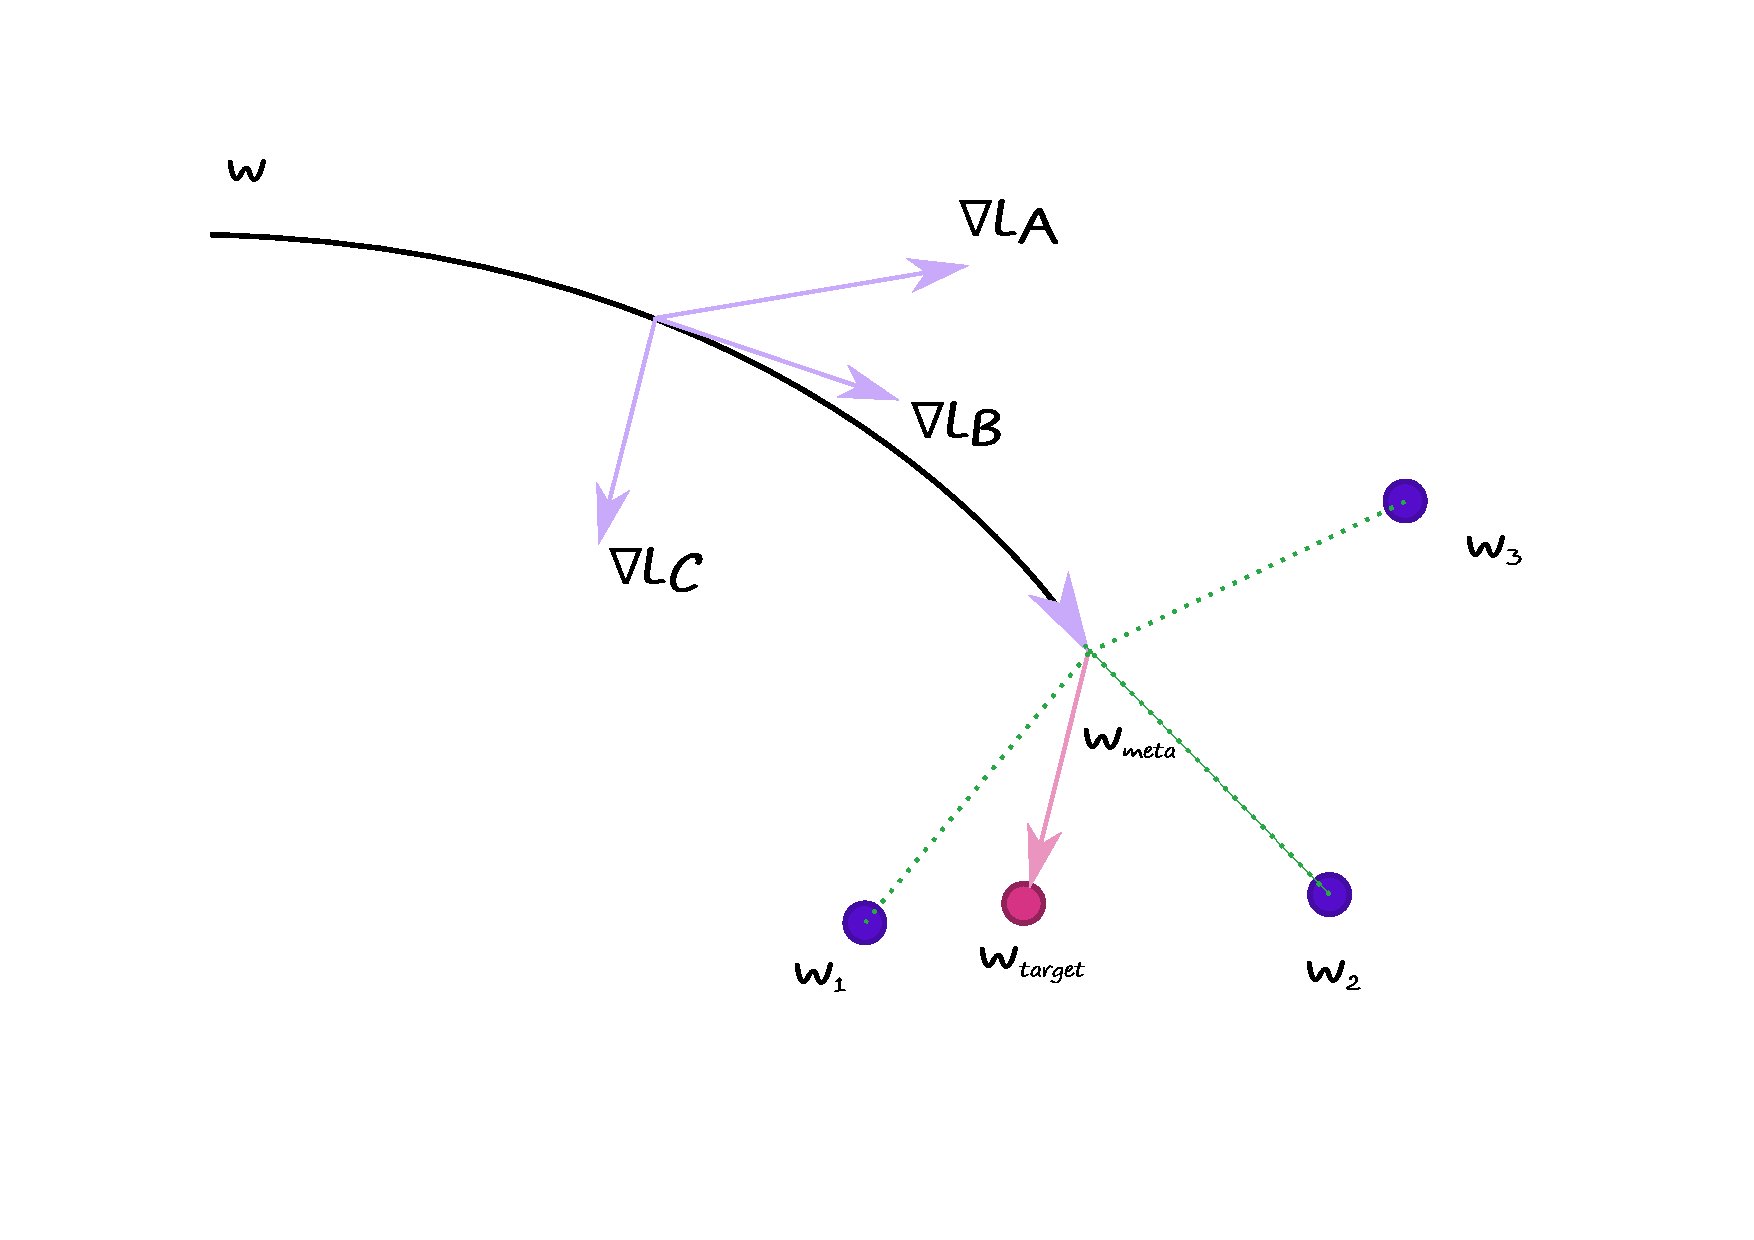
\includegraphics[width=\textwidth]{figures/maml}
}

\headerbox{3. Experimental Setup}{name=expr,column=0, below=intro, span=2}
{
  \begin{itemize}
    \color{Pink} \item \color{Black} Tasks: linear/nonlinear regression problems with noisy ($\varepsilon  \sim \mathcal{N}(0, \sigma^2)$) observations of functions $f(\mathbf{x})$
      \begin{equation}\label{eq:task}
    \mathbf{y}= f(\mathbf{x})+\varepsilon, 
  \end{equation}  

  \begin{center}
  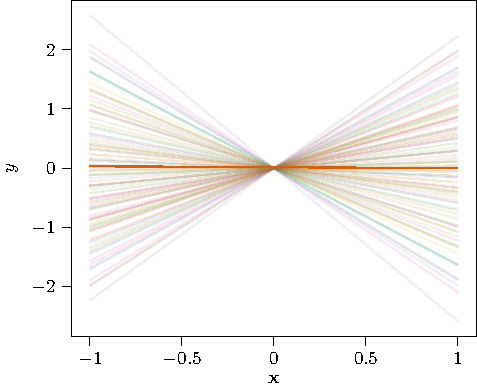
\includegraphics[width=0.31\textwidth]{lin_maml.pdf}%
  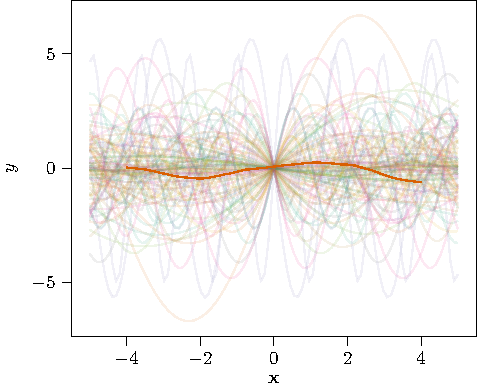
\includegraphics[width=0.31\textwidth]{nonlin_maml.pdf}
  \end{center}
\color{Pink} \item \color{Black} Estimator: model $\hat{M}$ trained  with a given dataset $\mathcal{Z}:=\{\mathbf{x}_i, y_i\}_{i=0}^{N}$
  \color{Pink} \item \color{Black} Performance: expected error over the task distribution $p_\mathcal{T}$ and data distribution $p_\mathcal{Z}$
  \begin{equation}\label{eq:ee}
    \mathcal{E}:= \iiint(\mathcal{\hat{M}}(\mathbf{x}) - y)^2 p(\mathbf{x}, y)p_{\mathcal{Z}} p_{\mathcal{T}} d\mathbf{x} dy d\mathcal{Z} d\mathcal{T}
  \end{equation}
  \end{itemize}
  
}

\headerbox{4. Baselines}{name=other,column=2, below=maml, span=1}
{
  \begin{itemize}
    \color{Pink} \item \color{Black} Linear/Kernelized Ridge Regression
    \color{Pink} \item \color{Black} Randomly Initialized Gradient Descent
  \end{itemize}
  \begin{center}
  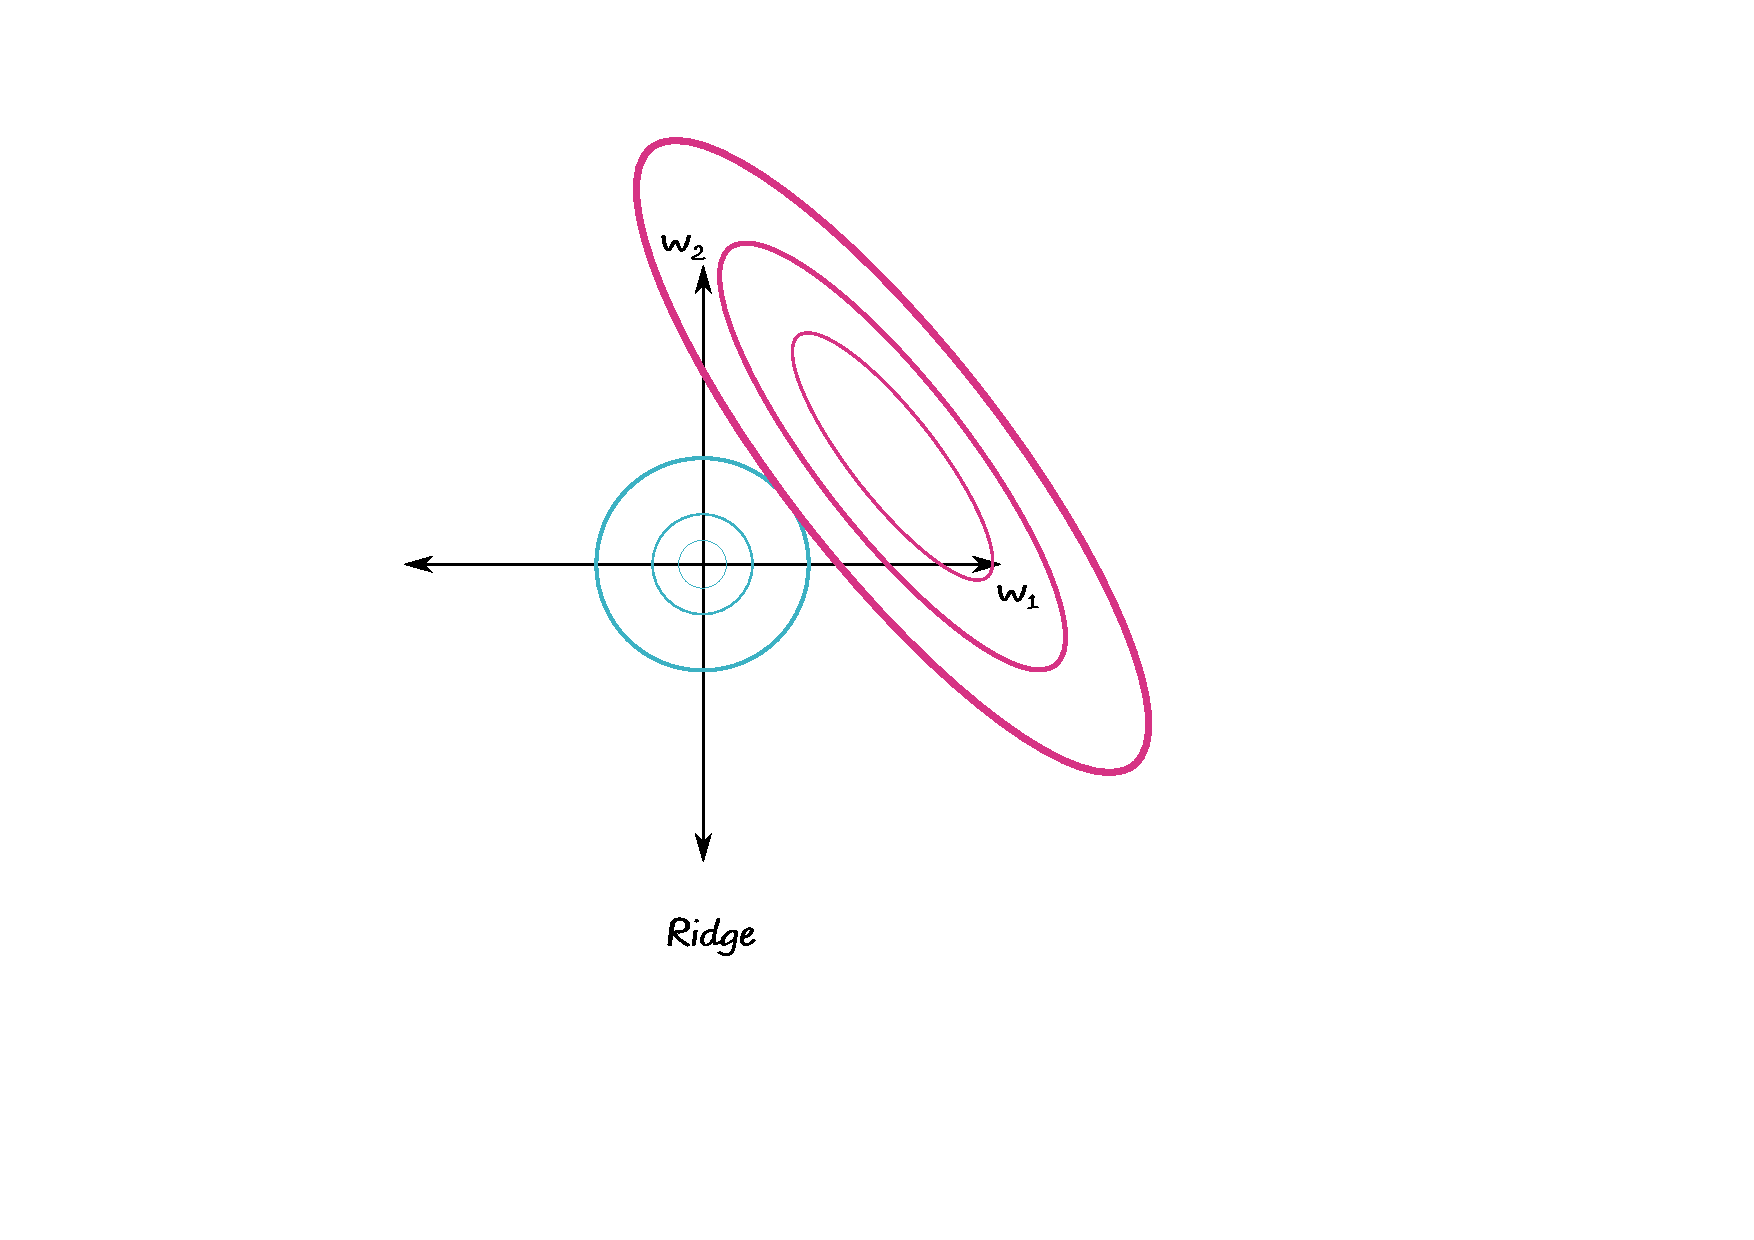
\includegraphics[width=1.2\textwidth]{figures/ridge}
  \end{center}
}

\headerbox{5. Results for Task Variances $c$ and $c_2$ ( $N = 1, \quad 10, \quad  50$ )
}{name=res,column=0, below=expr, span=2}
{
  \begin{itemize}
    \color{Pink} \item \color{Black} Linear problem: $f(\mathbf{x}):=\mathbf{x}^\text{T}\mathbf{a}$

  \end{itemize}

  \begin{center}
  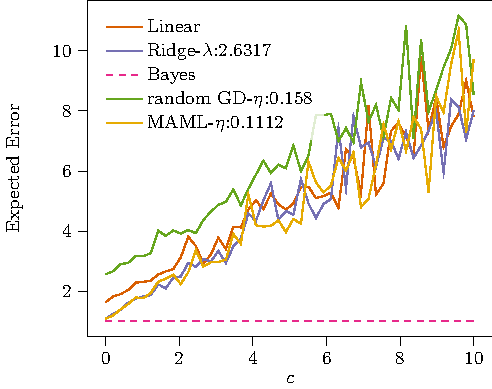
\includegraphics[width=0.31\textwidth]{lin_c_1.pdf}%
  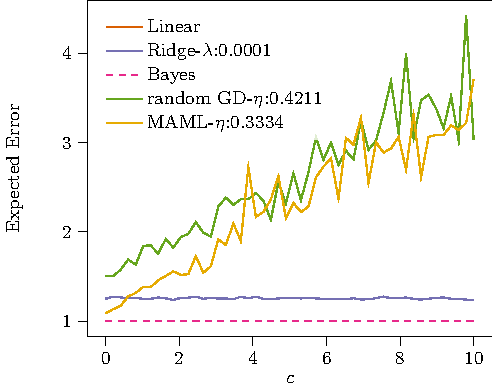
\includegraphics[width=0.31\textwidth]{lin_c_2.pdf}%
  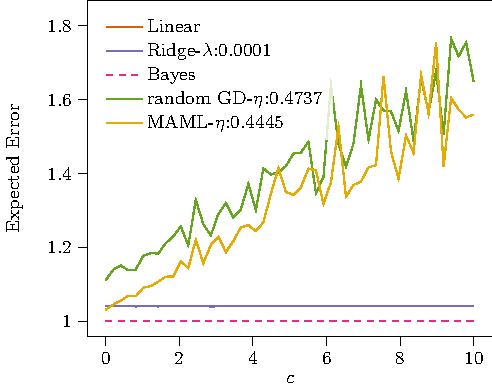
\includegraphics[width=0.31\textwidth]{lin_c_3.pdf}%
  \end{center}

  \begin{itemize}
    \color{Pink} \item \color{Black} Nonlinear problem: $f(\mathbf{x}):=\text{sin}(\mathbf{x}+\boldsymbol{\phi})^{\text{T}}\mathbf{a}$

  \end{itemize}

  \begin{center}
  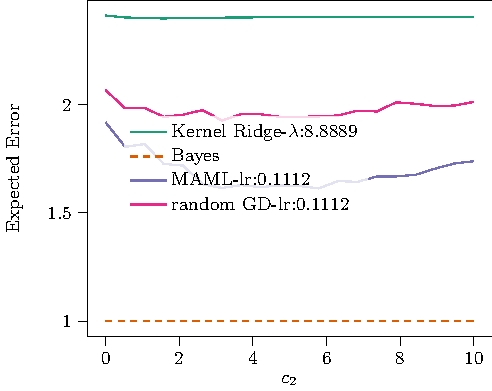
\includegraphics[width=0.31\textwidth]{nonlin_c_1.pdf}%
  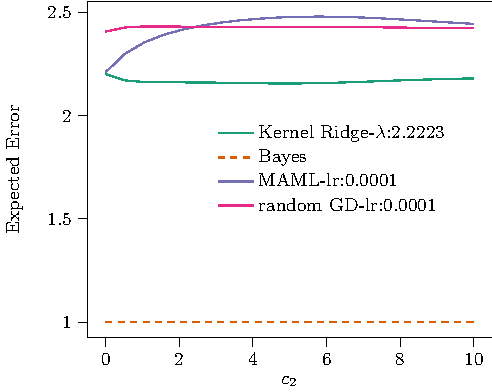
\includegraphics[width=0.31\textwidth]{nonlin_c_2.pdf}%
  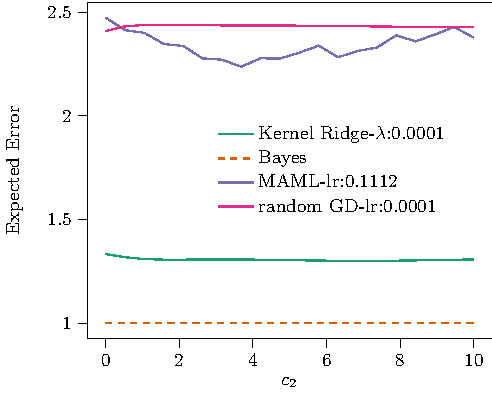
\includegraphics[width=0.31\textwidth]{nonlin_c_3.pdf}%
  \end{center}

}

\headerbox{6. Conclusions}{name=conc,column=2, below=other, span=1}
{
  \begin{itemize}
    \color{Pink} \item \color{Black} Given enough data single-task learners can outperform MAML in expectation in most the cases
    \color{Pink} \item \color{Black} Task variance highly influences the performance of MAML in expectation.
  \end{itemize}
}


\headerbox{8. References}{name=ref,column=0, below=res, span=3}
{
\renewcommand{\section}[2]{\vskip 0.05em} % Get rid of the default "References" section title
%%\nocite{*} % Insert publications even if they are not cited in the poster
\bibliographystyle{unsrt}  
\small\bibliography{/home/taylanot/Dropbox/archive_bib/mylibrary.bib}   
}
\headerbox{7. Experimentation}{name=future,column=2, below=conc, span=1}
{
  \begin{center}
    
\includegraphics[scale=0.1]{logos/qrlogo2.pdf}
  \end{center}
}

%\headerbox{8. Future Directions}{name=future,column=2, below=conc, span=1}
%{
%  \begin{itemize}
%    \color{Pink} \item \color{Black} Does kkk
%  \end{itemize}
%}
\end{poster}

\end{document}
